\documentclass[12pt]{article}
\usepackage{amsmath}
\usepackage{graphicx}
\usepackage{hyperref}
\usepackage{listings}
\usepackage{color}
\usepackage{pythonhighlight}

\title{Operating System Course Report - First Half of the Semester}
\author{B class}
\date{\today}

\begin{document}

\maketitle
\newpage

\tableofcontents
\newpage

\section{Introduction}
This report summarizes the topics covered during the first half of the
Operating System course. It includes theoretical concepts, practical
implementations, and assignments. The course focuses on the fundamentals of
operating systems, including system architecture, process management, CPU
scheduling, and deadlock handling.

\section{Course Overview}
\subsection{Objectives}
The main objectives of this course are:
\begin{itemize}
    \item To understand the basic components and architecture of a computer system.
    \item To learn process management, scheduling, and inter-process communication.
    \item To explore file systems, input/output management, and virtualization.
    \item To study the prevention and handling of deadlocks in operating systems.
\end{itemize}

\subsection{Course Structure}
The course is divided into two halves. This report focuses on the first half,
which covers:
\begin{itemize}
    \item Basic Concepts and Components of Computer Systems
    \item System Performance and Metrics
    \item System Architecture of Computer Systems
    \item Process Description and Control
    \item Scheduling Algorithms
    \item Process Creation and Termination
    \item Introduction to Threads
    \item File Systems
    \item Input and Output Management
    \item Deadlock Introduction and Prevention
    \item User Interface Management
    \item Virtualization in Operating Systems
\end{itemize}

\section{Topics Covered}

\subsection{Basic Concepts and Components of Computer Systems}
This section explains the fundamental components that make up a computer
system, including the CPU, memory, storage, and input/output devices.

\subsection{System Performance and Metrics}
This section introduces various system performance metrics used to measure the
efficiency of a computer system, including throughput, response time, and
utilization.

\subsection{System Architecture of Computer Systems}
Describes the architecture of modern computer systems, focusing on the
interaction between hardware and the operating system.

\subsection{Process Description and Control}
Processes are a central concept in operating systems. This section covers:
\begin{itemize}
    \item Process states and state transitions
    \item Process control block (PCB)
    \item Context switching
\end{itemize}

\subsection{Scheduling Algorithms}
This section covers:
\begin{itemize}
    \item First-Come, First-Served (FCFS)
    \item Shortest Job Next (SJN)
    \item Round Robin (RR)
\end{itemize}
It explains how these algorithms are used to allocate CPU time to processes.

\subsection{Process Creation and Termination}
Details how processes are created and terminated by the operating system,
including:
\begin{itemize}
    \item Process spawning
    \item Process termination conditions
\end{itemize}

\subsection{Introduction to Threads}
This section introduces the concept of threads and their relation to processes,
covering:
\begin{itemize}
    \item Single-threaded vs. multi-threaded processes
    \item Benefits of multithreading
\end{itemize}

% \begin{figure}[h]
%     \centering
%     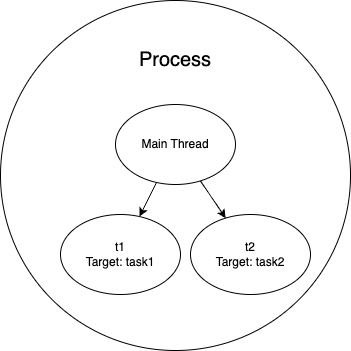
\includegraphics[width=0.5\textwidth]{./b_class/asset/example.png}  % Sesuaikan nama file dan ukurannya
%     \caption{Ini adalah gambar contoh dari multithreading.}
%     \label{fig:contoh_gambar}
% \end{figure}

Seperti yang terlihat pada Gambar \ref{fig:contoh_gambar}, inilah cara
menambahkan gambar dengan keterangan.

\subsection{File Systems}
File systems provide a way for the operating system to store, retrieve, and
manage data. This section explains:
\begin{itemize}
    \item File system structure
    \item File access methods
    \item Directory management
\end{itemize}

\subsection{Input and Output Management}
Input and output management is key for handling the interaction between the
system and external devices. This section includes:
\begin{itemize}
    \item Device drivers
    \item I/O scheduling
\end{itemize}

\subsection{Deadlock Introduction and Prevention}
Explores the concept of deadlocks and methods for preventing them:

\subsubsection{\textit{Deadlock conditions}}

\subsubsection{\textit{Deadlock prevention methods}}

\par  Pencegahan terhadap \textit{deadlock} adalah teknik yang digunakan untuk
mencegah sistem memasuki keadaan \textit{deadlock}. Berbeda dengan
\textit{deadlock} avoidance yang di mana mengatasi masalah setelah
\textit{deadlock} terjadi, pencegahan ada agar memperkecil kemungkinan
terjadinya \textit{deadlock}. Pencegahan \textit{deadlock} dapat dilakukan
dengan cara menghindari keadaan-keadaan yang dapat menyebabkan
\textit{deadlock}. Beberapa metode pencegahan \textit{deadlock} adalah:

\begin{enumerate}
    \item \textit{Resources Ordering}

          \par \textit{Resources Ordering} adalah pengurutan sumber daya di mana setiap sumber daya
          dalam sistem diberi nomor atau urutan unik. Proses harus meminta sumber daya
          dalam urutan yang konsisten dengan nomor tersebut. Artinya, jika suatu proses
          sudah memegang satu sumber daya dengan nomor lebih rendah, maka ia hanya boleh
          meminta sumber daya dengan nomor lebih tinggi.

          \par Salah satu contoh kasus pencegahan \textit{deadlock} dengan metode
          \textit{resources ordering} yaitu jika ada dua sumber daya, R1 dan R2, dan
          proses P1 memegang R1 dan ingin meminta R2, maka metode ini memastikan bahwa
          proses P1 tidak dapat memegang R2 tanpa mengikuti urutan yang telah ditentukan.

    \item \textit{Resource allocation denial}

          \par Metode ini dikenal juga sebagai \textit{Banker's Algorithm} atau \textit{safety
              algorithm}, di mana sistem memeriksa apakah pemberian sumber daya tertentu akan
          menyebabkan kondisi \textit{unsafe} atau potensi \textit{deadlock}. Jika
          pemberian sumber daya dianggap tidak aman, maka permintaan sumber daya tersebut
          akan ditolak.

          \par Metode \textit{resources allocation denial} adalah ketika proses P1 meminta
          sumber daya R1. Sebelum mengalokasikan sumber daya, sistem mengevaluasi apakah
          proses lain bisa menyelesaikan eksekusi dengan sumber daya yang tersisa. Jika
          tidak, permintaan P1 ditolak sementara waktu dan akan dilanjutkan ketika semua
          sumber daya yang dibutuhkan sudah lengkap.

    \item \textit{Timeouts}

          \par Dalam metode ini, sistem menggunakan batas waktu (\textit{timeout}) untuk
          menunggu sumber daya. Jika proses menunggu terlalu lama, ia akan dipaksa gagal
          atau \textit{restart}. \textit{Timeout} dapat digunakan untuk mencegah proses
          berlama-lama dalam kondisi menunggu, sehingga menghindari \textit{deadlock}.

          \par Proses P1 sedang menunggu sumber daya R1 selama lima menit. Jika setelah batas
          waktu ini R1 belum tersedia, proses P1 akan dibatalkan atau dijadwalkan ulang
          untuk mencoba lagi.

    \item \textit{Avoidance of hold-and-wait conditions}

          \par Teknik \textit{avoidance of hold-and-wait conditions} adalah teknik pencegahan
          \textit{deadlock} dengan kondisi saling tunggu sumber daya antara suatu proses.
          Dalam teknik ini, proses tidak diperbolehkan menahan sumber daya sambil
          menunggu sumber daya lain. Proses harus meminta semua sumber daya yang
          dibutuhkan di awal (sebelum memulai eksekusi) atau melepaskan sumber daya yang
          sedang dipegang sebelum meminta sumber daya tambahan.

          \par Dalam penerapannya, Proses P1 harus meminta sumber daya R1 dan R2 sekaligus.
          Jika R2 tidak tersedia, maka proses tidak diperbolehkan memegang R1 dan harus
          melepaskannya sampai kedua sumber daya tersedia. Setiap proses yang belum
          memiliki sumber daya yang cukup untuk berjalan maka akan terus menunggu hingga
          sumber daya yang dibutuhkan terpenuhi semua.

    \item \textit{Resource preemption}

          \par Teknik ini memungkinkan sistem untuk merebut atau mengambil kembali sumber daya
          dari proses yang sedang berjalan jika diperlukan oleh proses lain yang lebih
          prioritas atau jika diperlukan untuk mencegah
          \textit{deadlock}\textit{deadlock}.

          \par Dalam kasus seperti proses P1 harus meminta sumber daya R1 dan R2 sekaligus.
          Jika R2 tidak tersedia, proses tidak diperbolehkan memegang R1 dan harus
          melepaskannya sampai kedua sumber daya tersedia.
\end{enumerate}

\subsection{User Interface Management}
This section discusses the role of the operating system in managing the user
interface. Topics covered include:
\begin{itemize}
    \item Graphical User Interface (GUI)
    \item Command-Line Interface (CLI)
    \item Interaction between the user and the operating system
\end{itemize}

\subsection{Virtualization in Operating Systems}
Virtualization allows multiple operating systems to run concurrently on a
single physical machine. This section explores:
\begin{itemize}
    \item Concept of virtualization
    \item Hypervisors and their types
    \item Benefits of virtualization in modern computing
\end{itemize}

\section{Assignments and Practical Work}
\subsection{Assignment 1: Process Scheduling}
Students were tasked with implementing various process scheduling algorithms
(e.g., FCFS, SJN, and RR) and comparing their performance under different
conditions.

\subsubsection{Kelompok 11}
\begin{python}
    import heapq

    class Process:
        def __init__(self, id, arrival_time, burst_time):
            self.id = id
            self.arrival_time = arrival_time
            self.burst_time = burst_time
    
    def sjf_scheduling(processes):
        time = 0
        completed = []
        ready_queue = []
        processes.sort(key=lambda x: x.arrival_time)
    
        while processes or ready_queue:
            print(f"\Waktu saat ini: {time}")
            
            while processes and processes[0].arrival_time <= time:
                arriving_process = processes.pop(0)
                print(f"Process {arriving_process.id} tiba saat {arriving_process.arrival_time}")
                heapq.heappush(ready_queue, (arriving_process.burst_time, arriving_process.id, arriving_process))
            
            if ready_queue:
                _, _, current_process = heapq.heappop(ready_queue)
                print(f"Menjalankan process {current_process.id} dengan burst time {current_process.burst_time}")
                time += current_process.burst_time
                completed.append((current_process.id, time))
                print(f"Process {current_process.id} selesai di {time}")
            else:
                next_arrival = processes[0].arrival_time
                time = next_arrival
    
        return completed
    
    processes = [
        Process(1, 0, 10),
        Process(2, 1, 6),
        Process(3, 3, 2),
        Process(4, 5, 4)
    ]
    
    result = sjf_scheduling(processes)
\end{python}

\textbf{Soal :}
\\
Dari kode python diatas, Tuliskan output yang dihasilkan dan gambarkan eksekusi proses menggunakan Grantt chart!

\textbf{Jawaban :}
\begin{python}
Waktu saat ini: 0
Process 1 tiba saat 0
Menjalankan process 1 dengan burst time 10
Process 1 selesai di 10

Waktu saat ini: 10
Process 2 tiba saat 1
Process 3 tiba saat 3
Process 4 tiba saat 5
Menjalankan process 3 dengan burst time 2
Process 3 selesai di 12

Waktu saat ini: 12
Menjalankan process 4 dengan burst time 4
Process 4 selesai di 16

Waktu saat ini: 16
Menjalankan process 2 dengan burst time 6
Process 2 selesai di 22

\end{python}

\renewcommand{\figurename}{Gambar}
\begin{figure}[h]
    \centering
    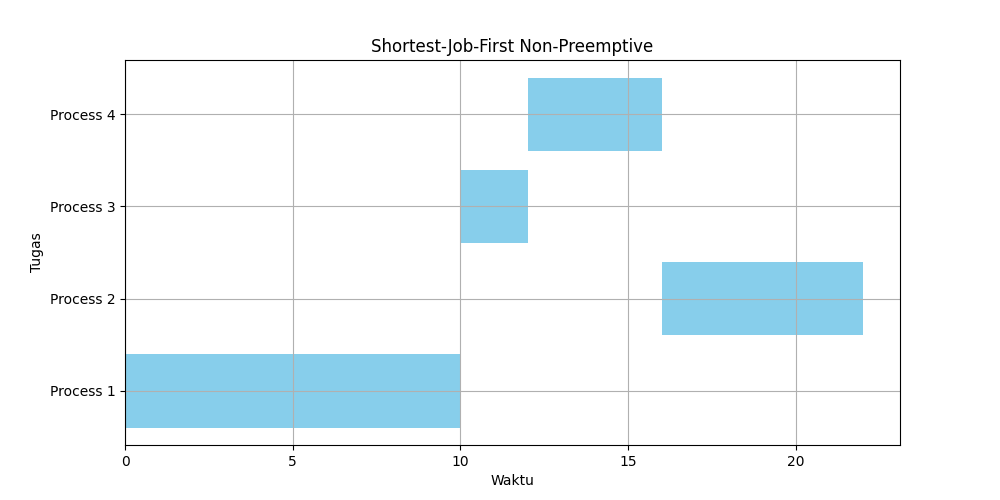
\includegraphics[width=14cm]{./asset/GranttChart.png}
    \caption{Shortest-Job-First Process Scheduling}
\end{figure}
% \subsubsection{Group 1}
% \begin{python}
%     class Process:
%     def __init__(self, pid, arrival_time, burst_time):
%     self.pid = pid
%     self.arrival_time = arrival_time
%     self.burst_time = burst_time
%     self.completion_time = 0
%     self.turnaround_time = 0
%     self.waiting_time = 0
% \end{python}

% \begin{table}[htbp] % Optional: For floating position
%     \centering
%     \begin{tabular}{|c|c|c|} % Defines number of columns and alignment (c = center, l = left, r = right). '|' creates vertical lines.
%         \hline
%         Header 1        & Header 2        & Header 3        \\ % Column headers
%         \hline
%         Row 1, Column 1 & Row 1, Column 2 & Row 1, Column 3 \\ % First row of data
%         \hline
%         Row 2, Column 1 & Row 2, Column 2 & Row 2, Column 3 \\ % Second row of data
%         \hline
%     \end{tabular}
%     \caption{Your table caption} % Optional: For adding a caption
%     \label{tab:your_label} % Optional: For cross-referencing the table

% \end{table}
\subsection{Assignment 2: Deadlock Handling}
In this assignment, students were asked to simulate different deadlock
scenarios and explore various prevention methods.

\subsubsection{Kelompok 11}
\begin{python}
    import numpy as np

    class DeadlockPrevention:
    def __init__(self, available, max_need, allocation):
        self.available = np.array(available)
        self.max_need = np.array(max_need)
        self.allocation = np.array(allocation)
        self.need = self.max_need - self.allocation

    def is_safe_state(self):
        work = self.available.copy()
        finish = [False] * len(self.allocation)
        
        while False in finish:
            safe = False
            for i in range(len(finish)):
                if not finish[i] and all(self.need[i] <= work):
                    work += self.allocation[i]
                    finish[i] = True
                    safe = True
            if not safe:
                return False
        return True

    def request_resources(self, process, request):
        if any(request > self.need[process]):
            return False
        if any(request > self.available):
            return False
        
        self.available -= request
        self.allocation[process] += request
        self.need[process] -= request
        
        if self.is_safe_state():
            return True
        
        self.available += request
        self.allocation[process] -= request
        self.need[process] += request
        return False

    # Inisialisasi sistem
    available = [3, 3, 2]
    max_need = [
    [7, 5, 3],
    [3, 2, 2],
    [9, 0, 2],
    [2, 2, 2],
    [4, 3, 3]
    ]
    allocation = [
    [0, 1, 0],
    [2, 0, 0],
    [3, 0, 2],
    [2, 1, 1],
    [0, 0, 2]
    ]

    dp = DeadlockPrevention(available, max_need, allocation)

    # Simulasi permintaan sumber daya
    print("Initial state is safe:", dp.is_safe_state())

    request1 = [1, 0, 2]
    process1 = 1
    print(f"Request {request1} for process {process1} granted:", dp.request_resources(process1, request1))
    
    request2 = [3, 3, 0]
    process2 = 4
    print(f"Request {request2} for process {process2} granted:", dp.request_resources(process2, request2))
    
    print("Final state is safe:", dp.is_safe_state())
    
\end{python}

\textbf{Soal :}

\par Analisis kode Python di atas yang mengimplementasikan algoritma \textit{resources allocation denial} untuk
pencegahan \textit{deadlock}. Jelaskan alur kerja kode, fungsi utama dari setiap metode,
bagaimana kode ini mencegah \textit{deadlock}, dan prediksi outputnya beserta alasannya.

\textbf{Jawaban :}

\begin{enumerate}
    \item Alur kerja dan fungsi utama
    
Implementasi metode \textit{resources allocation denial} dalam kode ini berpusat pada kelas \texttt{DeadlockPrevention}. Kelas ini menginisialisasi sistem dengan informasi tentang sumber daya yang tersedia, kebutuhan maksimum setiap proses, dan alokasi saat ini. Metode utama dalam kelas ini adalah \texttt{is\_safe\_state()} dan \texttt{request\_resources()}.

Metode \texttt{is\_safe\_state()} berperan krusial dalam pencegahan \textit{deadlock}. Metode ini mensimulasikan eksekusi semua proses untuk memastikan bahwa setidaknya ada satu urutan eksekusi yang memungkinkan semua proses untuk menyelesaikan tugasnya. Ini dilakukan dengan menggunakan array \texttt{work} untuk melacak sumber daya yang tersedia selama simulasi dan mencoba untuk "menyelesaikan" setiap proses secara berurutan. Jika semua proses dapat diselesaikan, keadaan sistem dianggap aman.

Di sisi lain, metode \texttt{request\_resources()} menangani permintaan sumber daya dari proses. Metode ini pertama-tama memeriksa validitas permintaan, memastikan bahwa permintaan tidak melebihi kebutuhan proses atau sumber daya yang tersedia. Jika permintaan valid, metode ini mencoba mengalokasikan sumber daya dan kemudian memeriksa keamanan sistem menggunakan \texttt{is\_safe\_state()}. Jika alokasi menyebabkan keadaan tidak aman, perubahan dibatalkan dan permintaan ditolak, efektif mencegah sistem memasuki keadaan yang berpotensi \textit{deadlock}.

\item Mekanisme Pencegahan \textit{Deadlock}

metode \textit{resources allocation denial} mencegah \textit{deadlock} dengan menerapkan beberapa prinsip kunci. Pertama, ia selalu memeriksa keamanan sistem sebelum mengalokasikan sumber daya. Ini memastikan bahwa sistem tidak pernah memasuki keadaan yang dapat mengarah pada deadlock. Kedua, algoritma ini hanya mengizinkan alokasi sumber daya jika alokasi tersebut tidak menyebabkan keadaan tidak aman, secara efektif mencegah kondisi {hold-and-wait}. Ketiga, dengan memastikan bahwa setiap alokasi sumber daya tidak mengarah pada siklus ketergantungan, algoritma ini secara implisit mencegah \textit{circular wait}, salah satu kondisi yang diperlukan untuk terjadinya deadlock.

\item Analisis Output

Berdasarkan kode yang diberikan, output yang diharapkan adalah:

\begin{verbatim}
Initial state is safe: True
Request [1, 0, 2] for process 1 granted: True
Request [3, 3, 0] for process 4 granted: False
Final state is safe: True
\end{verbatim}

Output ini menunjukkan bahwa keadaan awal sistem aman, yang berarti distribusi sumber daya awal memungkinkan semua proses untuk menyelesaikan eksekusinya. Permintaan pertama ([1, 0, 2] untuk proses 1) diterima karena setelah alokasi, sistem tetap dalam keadaan aman. Namun, permintaan kedua ([3, 3, 0] untuk proses 4) ditolak karena akan menghabiskan terlalu banyak sumber daya dan berpotensi menyebabkan deadlock. Keadaan akhir sistem tetap aman karena hanya permintaan yang aman yang diterima.
\end{enumerate}


\subsection{Assignment 3: Multithreading and Amdahl's Law}
This assignment involved designing a multithreading scenario to solve a
computationally intensive problem. Students then applied **Amdahl's Law** to
calculate the theoretical speedup of the program as the number of threads
increased.

\subsection{Assignment 4: Simple Command-Line Interface (CLI) for User Interface Management}
Students were tasked with creating a simple **CLI** for user interface
management. The CLI should support basic commands such as file manipulation
(creating, listing, and deleting files), process management, and system status
reporting.

\subsection{Assignment 5: File System Access}
In this assignment, students implemented file system access routines,
including:
\begin{itemize}
    \item File creation and deletion
    \item Reading from and writing to files
    \item Navigating directories and managing file permissions
\end{itemize}

\subsubsection{Kelompok 11}
\textbf{Soal :}
Buatlah sebuah program Python sederhana yang melakukan operasi-operasi berikut:

\begin{enumerate}
    \item Membuat file bernama "contoh.txt" dengan isi "Ini adalah contoh isi file."
    \item Membaca dan menampilkan isi file "contoh.txt"
    \item Membuat direktori baru bernama "folder\_baru"
    \item Menampilkan isi direktori saat ini
    \item Mengubah izin file "contoh.txt" menjadi rw-r--r-- (644 dalam oktal)
    \item Menghapus file "contoh.txt" dan direktori "folder\_baru"
    \item Menampilkan kembali isi direktori saat ini
\end{enumerate}

\textbf{Jawaban :}
\begin{python}
import os
import shutil

def buat_file(nama_file, isi):
    with open(nama_file, 'w') as f:
        f.write(isi)
    print(f"File '{nama_file}' berhasil dibuat.")

def baca_file(nama_file):
    with open(nama_file, 'r') as f:
        isi = f.read()
    print(f"Isi file '{nama_file}':\n{isi}")

def hapus_file(nama_file):
    os.remove(nama_file)
    print(f"File '{nama_file}' berhasil dihapus.")

def buat_direktori(nama_dir):
    os.mkdir(nama_dir)
    print(f"Direktori '{nama_dir}' berhasil dibuat.")

def ubah_izin_file(nama_file, mode):
    os.chmod(nama_file, mode)
    print(f"Izin file '{nama_file}' berhasil diubah.")

def tampilkan_isi_direktori(path='.'):
    print(f"Isi direktori '{path}':")
    for item in os.listdir(path):
        print(item)

# Contoh penggunaan
if __name__ == "__main__":
    buat_file("contoh.txt", "Ini adalah contoh isi file.")
    baca_file("contoh.txt")
    
    buat_direktori("folder_baru")
    tampilkan_isi_direktori()
    
    ubah_izin_file("contoh.txt", 0o644)  # rw-r--r--
    
    hapus_file("contoh.txt")
    shutil.rmtree("folder_baru")
    tampilkan_isi_direktori()
\end{python}

\section{Conclusion}
The first half of the course introduced core operating system concepts,
including process management, scheduling, multithreading, and file system
access. These topics provided a foundation for more advanced topics to be
covered in the second half of the course.

\begin{thebibliography}{9}
    \bibitem{dijkstra1965} Dijkstra, E.W. (1965). Cooperating sequential processes. In Programming Languages (pp. 43-112). Academic Press.
    \bibitem{duo}Duo, W., Jiang, X., Karoui, O., Guo, X., You, D., Wang, S., Ruan, Y. (2020). A deadlock prevention policy for a class of multithreaded software. IEEE Access, 8, 16676-16688.
\end{thebibliography}

\end{document}
